\documentclass[12pt,letterpaper]{exam}
\usepackage[lmargin=1in,rmargin=1in,tmargin=1in,bmargin=1in]{geometry}
\usepackage{../style/exams}

% -------------------
% Course & Exam Information
% -------------------
\newcommand{\course}{MAT 101: Exam 1}
\newcommand{\term}{Fall -- 2021}
\newcommand{\examdate}{10/15/2021}
\newcommand{\timelimit}{85 Minutes}

\setbool{hideans}{true} % Student: True; Instructor: False

% -------------------
% Content
% -------------------
\begin{document}

\examtitle
\instructions{Write your name on the appropriate line on the exam cover sheet. This exam contains \numpages\ pages (including this cover page) and \numquestions\ questions. Check that you have every page of the exam. Answer the questions in the spaces provided on the question sheets. Be sure to answer every part of each question and show all your work.} 
\scores
\bottomline
\newpage

% ---------
% Questions
% ---------
\begin{questions}

% Question 1
\question[8] Compute the following: \pspace
\begin{parts}
\part $50 + 50 - 25 \cdot 0 + 2 + 2=$ \vfill
\part $2 - 20/5 \cdot 3=$ \vfill
\part $10 + 5 \cdot 2^2 - 3=$ \vfill
\part $24/8 - 5(10 - 11)^3=$ \vfill
\end{parts}



\newpage



% Question 2
\question[8] Simplify the following, being sure to have no negative exponents in your expression. \pspace
\begin{parts}
\part $\dfrac{x^{-1}}{x^{-8}}=$ \vfill
\part $\dfrac{xy^7}{x^5y^2}=$ \vfill
\part $\dfrac{3x^2 y^{-3}}{12x^6 y^3}=$ \vfill
\part $\left( \dfrac{x^3}{y^{-2}} \right)^2=$ \vfill
\end{parts}



\newpage



% Question 3
\question[8] Compute the following, being sure to simplify your answer completely: \pspace
\begin{parts}
\part $2 - \dfrac{1}{3}=$ \vfill
\part $\dfrac{5}{6} - \dfrac{3}{4}=$ \vfill
\part $-\dfrac{14}{15} \cdot \dfrac{10}{21}=$ \vfill
\part $\dfrac{\phantom{-}\frac{8}{9}\phantom{-}}{\frac{4}{3}}=$ \vfill
\end{parts}



\newpage



% Question 4
\question[6] Write a mathematical expression that computes the following: \pspace
\begin{parts}
\item 26\% of 37 \vfill
\item 95\% of 10 \vfill
\item 140\% of 16 \vfill
\end{parts} \vfill



% Question 5
\question[6] Write a mathematical expression that computes the following: \pspace
\begin{parts}
\item 40 increased by 60\% \vfill
\item 71 decreased by 90\% \vfill
\item 65 increased by 120\% \vfill
\end{parts}



\newpage



% Question 6
\question[4] Convert the following decimal numbers to scientific notation: \pspace
\begin{parts}
\part $0.00125=$ \vfill
\part $796000=$ \vfill
\end{parts} \vfill



% Question 7
\question[4] Convert the following numbers in scientific notation to decimal notation: \pspace
\begin{parts}
\part $2.3 \cdot 10^5=$ \vfill
\part $5.7 \cdot 10^{-2}=$ \vfill
\end{parts}



\newpage



% Question 8
\question[6] Find the prime factorizations of the following integers: \pspace
\begin{parts}
\part $120=$ \vfill
\part $84=$ \vfill
\part $76=$ \vfill
\end{parts}



% Question 9
\question[8] Compute the following: \pspace
\begin{parts}
\part $\gcd(6,15)=$ \vfill
\part $\gcd(574\,938, 1\,815\,000)= \gcd(2^1 \cdot 3^5 \cdot 7^1 \cdot 13^2, 2^3 \cdot 3^1 \cdot 5^4 \cdot 11^2)=$ \vfill
\part $\lcm(8,10)=$ \vfill
\part $\lcm(574\,938, 1\,815\,000)= \lcm(2^1 \cdot 3^5 \cdot 7^1 \cdot 13^2, 2^3 \cdot 3^1 \cdot 5^4 \cdot 11^2)=$ \vfill
\end{parts}



\newpage



% Question 10
\question[6] Simplify the following as much as possible: \pspace
\begin{parts} 
\part $\sqrt{48}=$ \vfill
\part $\sqrt{90}=$ \vfill
\part $\sqrt[3]{2^6 \cdot 3^4 \cdot 5}=$ \vfill
\end{parts}



\newpage



% Question 11
\question[6] Consider the following relations below:

	\[
	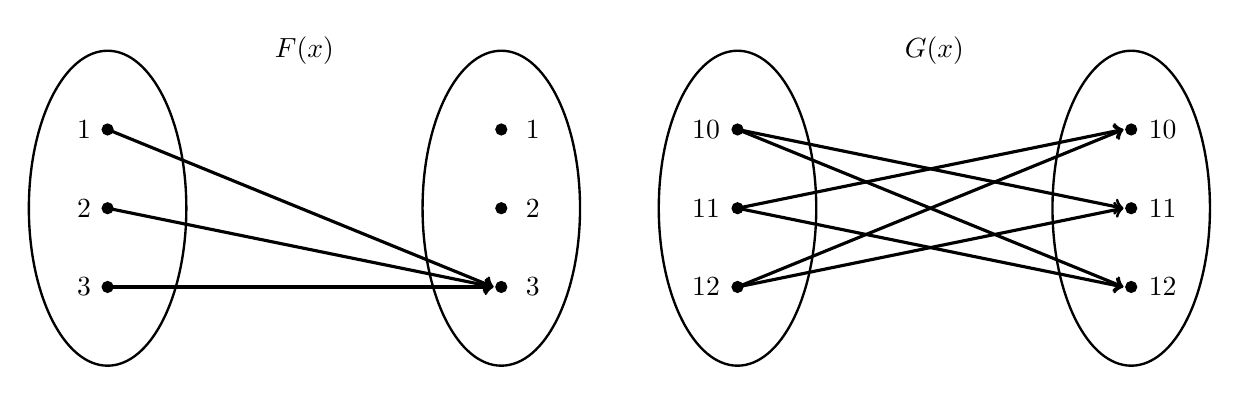
\begin{tikzpicture}
	\node at (2.5,2) {$F(x)$};
	% Ellipses
	\draw[line width=0.03cm] (0,0) circle (1 and 2);
	\draw[line width=0.03cm] (5,0) circle (1 and 2);
	
	% Nodes
	\draw[fill=black] (0,1) circle (0.07);
	\draw[fill=black] (0,0) circle (0.07);
	\draw[fill=black] (0,-1) circle (0.07);
	
	\draw[fill=black] (5,1) circle (0.07);
	\draw[fill=black] (5,0) circle (0.07);
	\draw[fill=black] (5,-1) circle (0.07);
	
	% Arrow
	\draw[line width=0.04cm,->] (0,1) -- (4.9,-1);
	\draw[line width=0.04cm,->] (0,0) -- (4.9,-1);
	\draw[line width=0.04cm,->] (0,-1) -- (4.9,-1);
	
	% Labels
	\node at (-0.3,1) {$1$};
	\node at (-0.3,0) {$2$};
	\node at (-0.3,-1) {$3$};
	
	\node at (5.4,1) {$1$};
	\node at (5.4,0) {$2$};
	\node at (5.4,-1) {$3$};
	
	\tikzset{shift={(8,0)}}
	%
	\node at (2.5,2) {$G(x)$};
	
	% Ellipses
	\draw[line width=0.03cm] (0,0) circle (1 and 2);
	\draw[line width=0.03cm] (5,0) circle (1 and 2);
	
	% Nodes
	\draw[fill=black] (0,1) circle (0.07);
	\draw[fill=black] (0,0) circle (0.07);
	\draw[fill=black] (0,-1) circle (0.07);
	
	\draw[fill=black] (5,1) circle (0.07);
	\draw[fill=black] (5,0) circle (0.07);
	\draw[fill=black] (5,-1) circle (0.07);
	
	% Arrow
	\draw[line width=0.04cm,->] (0,1) -- (4.9,0);
	\draw[line width=0.04cm,->] (0,1) -- (4.9,-1);
	\draw[line width=0.04cm,->] (0,0) -- (4.9,1);
	\draw[line width=0.04cm,->] (0,0) -- (4.9,-1);
	\draw[line width=0.04cm,->] (0,-1) -- (4.9,1);
	\draw[line width=0.04cm,->] (0,-1) -- (4.9,0);
	
	% Labels
	\node at (-0.4,1) {$10$};
	\node at (-0.4,0) {$11$};
	\node at (-0.4,-1) {$12$};
	
	\node at (5.4,1) {$10$};
	\node at (5.4,0) {$11$};
	\node at (5.4,-1) {$12$};
	\end{tikzpicture}
	\] \pspace

	\begin{minipage}[b]{0.49\textwidth}
	\centering
	\begin{tabular}{c|rcc|r}
	$x$ & $H(x)$ & \hspace{1cm} & $x$ & $J(x)$ \\ \cline{1-2} \cline{4-5}
	$1$ & $1$ & & $5$ & $-2$ \\
	$2$ & $1$ & & $6$ & $-1$ \\
	$3$ & $2$ & & $8$ & $0$ \\
	$4$ & $2$ & & $9$ & $1$ \\
	$5$ & $4$ & & $5$ & $2$
	\end{tabular}
	\end{minipage}
	\begin{minipage}[b]{0.49\textwidth}
	\[
	\begin{aligned}
	K(x)&:= 14x - 9 \\[0.6cm]
	L(x)&:= 5x(1 - x^3)
	\end{aligned}
	\]
	\end{minipage} \pvspace{0.6cm}
	
Determine if each of the relations given above is a function. If the relation is a function, write `T' (True) and if the relation is \emph{not} a function, write `F' (False): \pspace

	\begin{enumerate}[(a)]
	\item \uans{1.6cm}: $F(x)$ \pvspace{0.3cm}
	\item \uans{1.6cm}: $G(x)$ \pvspace{0.3cm}
	\item \uans{1.6cm}: $H(x)$ \pvspace{0.3cm}
	\item \uans{1.6cm}: $J(x)$ \pvspace{0.3cm}
	\item \uans{1.6cm}: $K(x)$ \pvspace{0.3cm}
	\item \uans{1.6cm}: $L(x)$
	\end{enumerate}



\newpage



% Question 12
\question[4] Consider the relation plotted below.
	\[
	\fbox{
	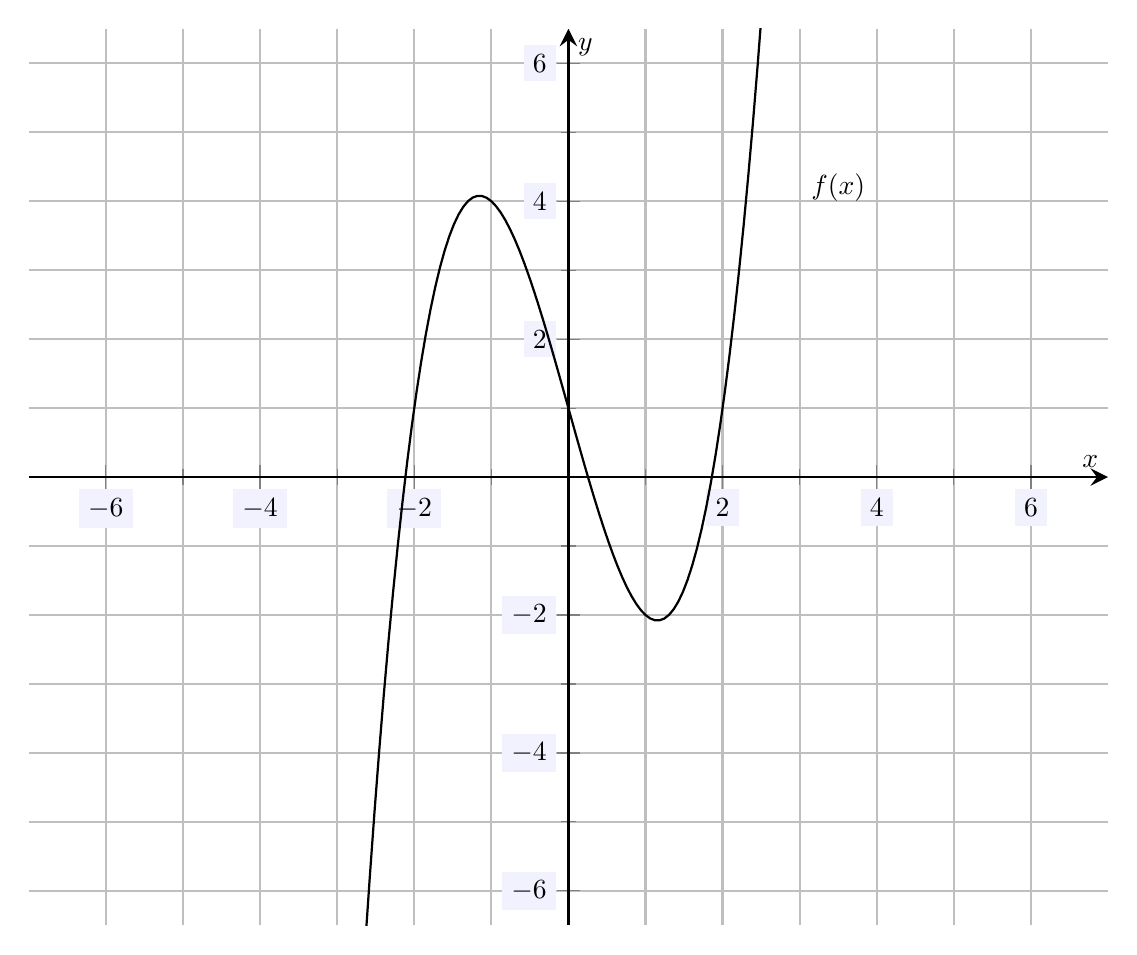
\begin{tikzpicture}[scale=2,every node/.style={scale=0.5}]
	\begin{axis}[
	grid=both,
	axis lines=middle,
	ticklabel style={fill=blue!5!white},
	xmin= -7, xmax=7,
	ymin= -6.5, ymax=6.5,
	xtick={-6,-4,-2,0,2,4,6},
	ytick={-6,-4,-2,0,2,4,6},
	minor tick = {-5,-3,...,5},
	xlabel=\(x\),ylabel=\(y\),
	]
	\node at (3.5,4.2) {$f(x)$};
	\addplot [domain= -3:3,samples=100] ({x},{x^3-4*x+1}); 
	\end{axis}
	\end{tikzpicture}
	}
	\] \pspace

\begin{parts}
\item Is the relation plotted above a function? Explain. \vfill
\item Does the relation above have an inverse function? Explain. \vfill
\end{parts}



\newpage



% Question 13
\question[10] Consider the functions given in the table below.
        \begin{table}[!ht]
        \centering
        \begin{tabular}{| c || c | c | c | c | c |} \hline
	$x$ & $-2$ & $-1$ & $0$ & $1$ & $2$ \\ \hline
	$f(x)$ & $3$ & $-2$ & $1$ & $6$ & $0$ \\ \hline
	$g(x)$ & $1$ & $2$ & $-1$ & $-2$ & $-6$ \\ \hline
        \end{tabular}
        \end{table}

Compute the following: \pspace
        \begin{enumerate}[(a)]
        \item $f(1)=$ \vfill
        \item $g(-1) - f(-2)=$ \vfill
        \item $f(-1)g(0)=$ \vfill
        \item $(f - g)(1)=$ \vfill
        \item $(f \circ g)(-2)=$ \vfill
        \item $(g \circ f)(2)=$ \vfill
        \item $y$-intercept of $g(x)$: \vfill
        \item $x$-intercept of $f(x)$: \vfill
        \end{enumerate}



\newpage



% Question 14
\question[8] Find the equation of the line through $(-4, 12)$ and $(2, 3)$.



\newpage



% Question 15
\question[8] Find the equation of the line that is perpendicular to $y= 6$ that passes through the $x$-intercept of $y= x - 3$. 






\end{questions}
\end{document}